% Options for packages loaded elsewhere
\PassOptionsToPackage{unicode}{hyperref}
\PassOptionsToPackage{hyphens}{url}
%
\documentclass[
]{article}
\usepackage{amsmath,amssymb}
\usepackage{iftex}
\ifPDFTeX
  \usepackage[T1]{fontenc}
  \usepackage[utf8]{inputenc}
  \usepackage{textcomp} % provide euro and other symbols
\else % if luatex or xetex
  \usepackage{unicode-math} % this also loads fontspec
  \defaultfontfeatures{Scale=MatchLowercase}
  \defaultfontfeatures[\rmfamily]{Ligatures=TeX,Scale=1}
\fi
\usepackage{lmodern}
\ifPDFTeX\else
  % xetex/luatex font selection
\fi
% Use upquote if available, for straight quotes in verbatim environments
\IfFileExists{upquote.sty}{\usepackage{upquote}}{}
\IfFileExists{microtype.sty}{% use microtype if available
  \usepackage[]{microtype}
  \UseMicrotypeSet[protrusion]{basicmath} % disable protrusion for tt fonts
}{}
\makeatletter
\@ifundefined{KOMAClassName}{% if non-KOMA class
  \IfFileExists{parskip.sty}{%
    \usepackage{parskip}
  }{% else
    \setlength{\parindent}{0pt}
    \setlength{\parskip}{6pt plus 2pt minus 1pt}}
}{% if KOMA class
  \KOMAoptions{parskip=half}}
\makeatother
\usepackage{xcolor}
\usepackage[margin=1in]{geometry}
\usepackage{longtable,booktabs,array}
\usepackage{calc} % for calculating minipage widths
% Correct order of tables after \paragraph or \subparagraph
\usepackage{etoolbox}
\makeatletter
\patchcmd\longtable{\par}{\if@noskipsec\mbox{}\fi\par}{}{}
\makeatother
% Allow footnotes in longtable head/foot
\IfFileExists{footnotehyper.sty}{\usepackage{footnotehyper}}{\usepackage{footnote}}
\makesavenoteenv{longtable}
\usepackage{graphicx}
\makeatletter
\def\maxwidth{\ifdim\Gin@nat@width>\linewidth\linewidth\else\Gin@nat@width\fi}
\def\maxheight{\ifdim\Gin@nat@height>\textheight\textheight\else\Gin@nat@height\fi}
\makeatother
% Scale images if necessary, so that they will not overflow the page
% margins by default, and it is still possible to overwrite the defaults
% using explicit options in \includegraphics[width, height, ...]{}
\setkeys{Gin}{width=\maxwidth,height=\maxheight,keepaspectratio}
% Set default figure placement to htbp
\makeatletter
\def\fps@figure{htbp}
\makeatother
\setlength{\emergencystretch}{3em} % prevent overfull lines
\providecommand{\tightlist}{%
  \setlength{\itemsep}{0pt}\setlength{\parskip}{0pt}}
\setcounter{secnumdepth}{-\maxdimen} % remove section numbering
\ifLuaTeX
  \usepackage{selnolig}  % disable illegal ligatures
\fi
\usepackage{bookmark}
\IfFileExists{xurl.sty}{\usepackage{xurl}}{} % add URL line breaks if available
\urlstyle{same}
\hypersetup{
  pdftitle={SPIDER LAB GIFTS},
  pdfauthor={Juan Jesús Oteros Rojas y Zaira Moreno Martín},
  hidelinks,
  pdfcreator={LaTeX via pandoc}}

\title{SPIDER LAB GIFTS}
\author{Juan Jesús Oteros Rojas y Zaira Moreno Martín}
\date{2024-12-15}

\begin{document}
\maketitle

{
\setcounter{tocdepth}{2}
\tableofcontents
}
\subsection{1. Introducción}\label{introducciuxf3n}

En la especie de araña \emph{Pisaura mirabilis}, las arañas machos se
casan con las arañas hembras para que se apareen dándoles regalos
envueltos en seda. Los regalos nupciales, que consisten en donaciones de
sustancias nutritivas por parte de los machos hacia las hembras. Estos
regalos pueden tener varias funciones: atraer a las hembras, asegurar la
transferencia de esperma e incluso actuar como inversión parental a
través de los recursos nutricionales proporcionados.\\
En esta especie en concreto se observa que a veces las arañas machos
hacen trampa. En lugar de envolver la comida en seda, envuelven algo
más, como trozos de una planta o un exoesqueleto de insecto vacío del
que ya han comido permitiendo a los machos ahorrar energía para su
propio beneficio reproductivo.\footnote{Ghislandi PG, Beyer M, Velado P,
  Tuni C (2017). La envoltura de seda de los regalos nupciales ayuda al
  comportamiento engañoso en las arañas masculinas. Ecología conductual
  28 (3), 744-749. \url{https://doi.org/10.1093/beheco/arx028}}

\subsection{2. Materiales y Métodos}\label{materiales-y-muxe9todos}

Los datos de este proyecto fueron descargados desde
\href{https://www.kaggle.com/datasets/mexwell/spider-lab-gifts/data}{kaggle}.
En el proyecto se usaron 27 individuos macho de la especie \emph{Pisaura
mirabilis}.

\begin{longtable}[]{@{}
  >{\centering\arraybackslash}p{(\columnwidth - 8\tabcolsep) * \real{0.1404}}
  >{\centering\arraybackslash}p{(\columnwidth - 8\tabcolsep) * \real{0.1579}}
  >{\centering\arraybackslash}p{(\columnwidth - 8\tabcolsep) * \real{0.2544}}
  >{\centering\arraybackslash}p{(\columnwidth - 8\tabcolsep) * \real{0.1930}}
  >{\centering\arraybackslash}p{(\columnwidth - 8\tabcolsep) * \real{0.2544}}@{}}
\caption{Tabla 1: Vista general datos}\tabularnewline
\toprule\noalign{}
\begin{minipage}[b]{\linewidth}\centering
FOOD.TREATMENT
\end{minipage} & \begin{minipage}[b]{\linewidth}\centering
SILK.WEIGHT..mg.
\end{minipage} & \begin{minipage}[b]{\linewidth}\centering
TOT.WRAPPING.DURATION..sec.
\end{minipage} & \begin{minipage}[b]{\linewidth}\centering
MALE.CEPH.WIDTH..mm.
\end{minipage} & \begin{minipage}[b]{\linewidth}\centering
MALE.MASS.BEFORE.TRIAL..mg.
\end{minipage} \\
\midrule\noalign{}
\endfirsthead
\toprule\noalign{}
\begin{minipage}[b]{\linewidth}\centering
FOOD.TREATMENT
\end{minipage} & \begin{minipage}[b]{\linewidth}\centering
SILK.WEIGHT..mg.
\end{minipage} & \begin{minipage}[b]{\linewidth}\centering
TOT.WRAPPING.DURATION..sec.
\end{minipage} & \begin{minipage}[b]{\linewidth}\centering
MALE.CEPH.WIDTH..mm.
\end{minipage} & \begin{minipage}[b]{\linewidth}\centering
MALE.MASS.BEFORE.TRIAL..mg.
\end{minipage} \\
\midrule\noalign{}
\endhead
\bottomrule\noalign{}
\endlastfoot
WF & 0.111 & 169 & 4.580 & 135 \\
LF & 0.044 & 187 & 3.023 & 64 \\
LF & 0.043 & 150 & 3.570 & 68 \\
WF & 0.084 & 249 & 3.330 & 51 \\
WF & 0.185 & 576 & 4.790 & 144 \\
WF & 0.094 & 351 & 4.110 & 95 \\
WF & 0.140 & 529 & 3.666 & 90 \\
WF & 0.067 & 208 & 3.666 & 82 \\
WF & 0.123 & 456 & 3.520 & 74 \\
LF & 0.143 & 331 & 4.330 & 113 \\
\end{longtable}

\subsection{3. Hipótesis y Resultados}\label{hipuxf3tesis-y-resultados}

\textbf{H0: Afecta la dieta al tiempo de envoltura total.}\\
\textbf{H1: No afecta al tiempo de envoltura la dieta.}.

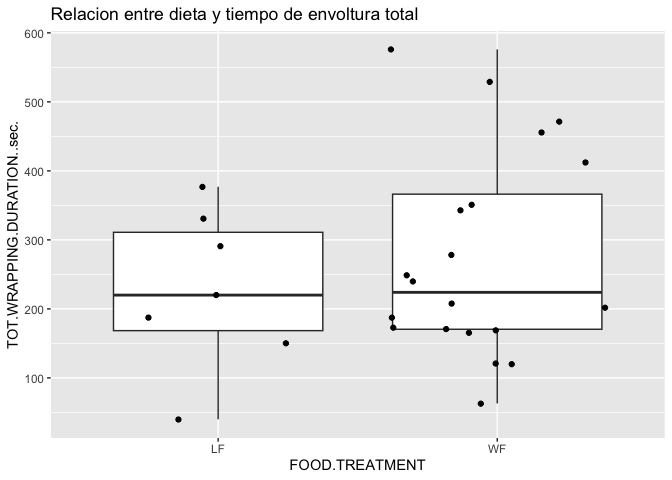
\includegraphics{ProyectoSpider_files/figure-latex/Relacion entre dieta y tiempo de envoltura-1.pdf}

En este caso se acepta \textbf{la hipótesis alternativa}, la dieta no
afecta al tiempo de envoltura porque vemos que el dato de la
\textbf{mediana} es similar en ambas dietas, la alta alimentacion
presenta \textbf{mayor dispersión} ya que presenta valores mas extremos
y por eso observamos que la caja es de mayor tamaño.

\newpage

\textbf{H0: Cambia la masa corporal masculina antes del experimento con
las diferentes dietas}\\
\textbf{H1: No cambia la masa corporal masculina antes del experimento
con las diferentes dietas}

\includegraphics{ProyectoSpider_files/figure-latex/Relación entre masa corporal masculina antes del experimento y dieta-1.pdf}

\textbf{H0: Cambia el ancho del céfalotorax con el tipo de dieta}\\
\textbf{H1: No Cambia el ancho del céfalotorax con el tipo de dieta}

\includegraphics{ProyectoSpider_files/figure-latex/Relación entre en ancho del céfalotorax y la dieta-1.pdf}

\textbf{H0: El tiempo de envoltura es mayor cuanto mayor peso tiene la
seda}\\
\textbf{H1: El peso de la seda no influye en el tiempo de envoltura}\\
\includegraphics{ProyectoSpider_files/figure-latex/Relación entre el tiempo de envoltura y el peso de la seda-1.pdf}

\textbf{H0: La dieta afecta al peso de la seda}\\
\textbf{H1: La dieta no afecta al peso de la seda}\\
\includegraphics{ProyectoSpider_files/figure-latex/Relación entre la dieta y el peso de la seda-1.pdf}

\end{document}
